
\documentclass[9pt]{pnas-new}
% Use the lineno option to display guide line numbers if required.
% Note that the use of elements such as single-column equations
% may affect the guide line number alignment. 

%\RequirePackage[english,slovene]{babel} % when writing in slovene
\RequirePackage[slovene,english]{babel} % when writing in english
\DeclareUnicodeCharacter{202F}{ }
\templatetype{pnasresearcharticle} % Choose template 
% {pnasresearcharticle} = Template for a two-column research article
% {pnasmathematics} = Template for a one-column mathematics article
% {pnasinvited} = Template for a PNAS invited submission

\selectlanguage{english}
%\etal{in sod.} % comment out when writing in english
%\renewcommand{\Authands}{ in } % comment out when writing in english
%\renewcommand{\Authand}{ in } % comment out when writing in english

\newcommand{\set}[1]{\ensuremath{\mathbf{#1}}}
\renewcommand{\vec}[1]{\ensuremath{\mathbf{#1}}}
\newcommand{\uvec}[1]{\ensuremath{\hat{\vec{#1}}}}
\newcommand{\const}[1]{{\ensuremath{\kappa_\mathrm{#1}}}} 
\usepackage{caption}
\usepackage{subcaption}
\usepackage{gensymb}
\usepackage{hyperref}
\newcommand{\num}[1]{#1}

\graphicspath{{./fig/}}

\title{Simulation of group behaviour during a protest}

% Use letters for affiliations, numbers to show equal authorship (if applicable) and to indicate the corresponding author
\author{Nik Čadež}
\author{Pedro Nuno Ferreira Moura de Macedo}
\author{Primož Mihelak}
\author{Luka Bajić}

\affil{Collective behaviour course research seminar report} 

% Please give the surname of the lead author for the running footer
\leadauthor{Čadež} 

\selectlanguage{english}

% Please add here a significance statement to explain the relevance of your work
\significancestatement{By conducting simulations of protests using various models for different subgroups of people, we hope to gain some insight into group behaviour during such events, that might make them logistically easier to organize/control in the future.}{Simulation | group behaviour | group dynamics}

\selectlanguage{english}

% Please include corresponding author, author contribution and author declaration information
%\authorcontributions{Please provide details of author contributions here.}
%\authordeclaration{Please declare any conflict of interest here.}
%\equalauthors{\textsuperscript{1}A.O.(Author One) and A.T. (Author Two) contributed equally to this work (remove if not applicable).}
%\correspondingauthor{\textsuperscript{2}To whom correspondence should be addressed. E-mail: author.two\@email.com}

% Keywords are not mandatory, but authors are strongly encouraged to provide them. If provided, please include two to five keywords, separated by the pipe symbol, e.g:
\keywords{Simulation | group behaviour | group dynamics} 

\begin{abstract}
The purpose of our project is to model the behaviour of a crowd during a protest as accurately as possible and attempt to observe the emerging behavioural patterns. At the start of a simulation we populate the scene with agents that belong in different subgroups (leader, protester, bystander), but eventually they can fluidly change between the groups based on various parameters, such as proneness to defection and recruitment. These parameters depend upon the distribution (in the sense of groups) of agents in an individual's field of view. The movement of the leader can either be manually controlled by the user, or determined by arbitrary goals within the topological map, while the other agents follow the leader when it appears in their field of vision, depending also on their aggression parameters. To give the simulation a practical use, we additionally allow the user to manually place police agents into the scene and observe how they impact the behaviour of the crowd. 
\end{abstract}

\dates{\textbf{\today}}
\program{BMA-RI}
\vol{2024/25}
\no{Group A} % group ID
%\fraca{FRIteza/201516.130}

\begin{document}

% Optional adjustment to line up main text (after abstract) of first page with line numbers, when using both lineno and twocolumn options.
% You should only change this length when you've finalised the article contents.
\verticaladjustment{-2pt}

\maketitle
\thispagestyle{firststyle}
\ifthenelse{\boolean{shortarticle}}{\ifthenelse{\boolean{singlecolumn}}{\abscontentformatted}{\abscontent}}{}

% If your first paragraph (i.e. with the \dropcap) contains a list environment (quote, quotation, theorem, definition, enumerate, itemize...), the line after the list may have some extra indentation. If this is the case, add \parshape=0 to the end of the list environment.
\dropcap{P}rotests are a widespread phenomenon involving typically large groups of people, oftentimes with different, or even conflicting goals between their respective subgroups. As such they are a fascinating subject for studies in various fields, from human psychology to group behaviour simulations, which was be our primary focus during the course of this project. 

\bigskip
The central idea for the project was inspired specifically by the 2020 protests in Ljubljana, that had a distinguishing feature of a prominent individual leader emerging and influencing the movement of the crowd, but we have attempted to make our model applicable more generally (for instance, with minor parameter adjustments, we should be able to easily model sports riots or other similar events with various subgroups).  

\section*{Related work}

Although there are many existing attempts to model protest behaviour, in terms of general structure, our project will primarily build on concepts proposed by Lemos, et. al. \cite{protests}. The basic idea is to split the agents into subgroups depending on their level of involvement with the protest. The proposed subgroups are:
\begin{itemize}
    \item active protesters, further divided by their level of aggression, 
    \item passive protesters - hereafter we refer to them as bystanders,
    \item police/crowd control agents: their primary goal is dispersing a crowd or redirecting it in a specific direction.
\end{itemize}

\bigskip
Clements and Fadai \cite{sportsriots} have developed a model that attempts to simulate emotional contagion in the context of a sports riot. Although our problem is slightly different in nature, we do apply the same principles of defection and recruitment in order to create approximately realistic transitions from active protesters to bystanders and vice versa, depending on what group the majority of agents in the current field of view of an individual belong to. 

\bigskip
To make simulations appear as realistic as possible, it is necessary to give all agents movement parameters that aim to mimic human behaviour in crowded environments. The forces that impact each agent are described, for instance by Itatani and Pelechano \cite{socialcrowdsimulation} and are divided into: collision avoidance force, wall repulsion force, end-position seeking force, group dynamics force and anticipatory collision avoidance force. 

\section*{Methods}

In this section we discuss our implementation of the crucial subproblems required to make the simulation appear as realistic as possible. 

\subsection*{Subgroups}
In addition to Lemos' subgroups \cite{protests}, we also implemented the concept of a leader and for this purpose we divided the simulation into two modes:
\begin{itemize}
    \item user manually controls the movement of a single leader: this can be used for instance to recreate very specific movement from real-life situations.
    \item multiple local leaders emerge spontaneously within the group and form a hierarchy of leaders.
\end{itemize}

\subsection*{Vision}
To give our agents awareness of their surroundings, we also need to model vision (example of a visualization is shown in figure \ref{vision}). This consists of two parts: 
\begin{itemize}
    \item field of view to model a human's eyesight. Default angle value is \begin{math}60\degree\end{math}, with a distance of 20 Unity units.
    \item peripersonal space to model a human's ability to feel a presence outside of their field of view, if the distance is small enough. Default angle value is \begin{math}360\degree\end{math}, with a distance of 1.7 Unity units.
\end{itemize}

\begin{figure}[H]
\centering
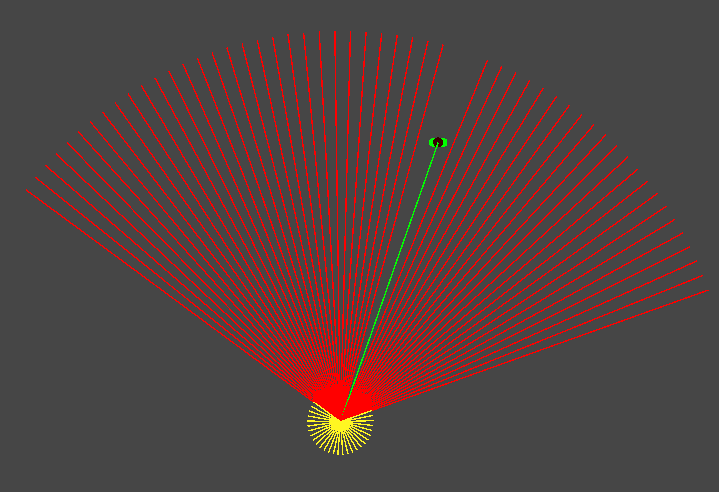
\includegraphics[width=0.95\columnwidth]{vision.png}
\caption{Visualization of the implemented vision: red rays represent field of vision, yellow rays represent peripersonal space, green ray represents a detected agent.}
\label{vision}
\end{figure}

Additionally, we created a function for agents to look around without changing their position (an equivalent of a human turning their head around to observe their surroundings), with a default value of \begin{math}300\degree\end{math} and a distance of 20 Unity units. This function is used in various scenarios, for instance when deciding on a suitable move position, or for a leader to determine how many active protesters surround it at a given moment. 

\subsection*{Movement}

Agents switch between two main states during the course of the simulation: standing still and in-motion. For this purpose we have come up with a restlessness parameter that gradually increases in agents that are standing still and once it reaches a certain threshold, the agent begins to move. To ensure that not all agents start and stop moving at the same time, it is paramount that the restlessness parameter is increased randomly (which based on our observations of various protest footage is the case for humans as well - perfectly synchronized behaviour is exceedingly rare). 

\bigskip
We deviate from Itatani \cite{socialcrowdsimulation} when it comes to End-Position-Seeking-Force, because the nature of our problem is considerably different. Our agents do not have an end position per se, therefore we have to set this value either to the position of the leader (in case a particular agent is currently following the leader), or an arbitrary nearby point in space (if an agent is not attached to the leader). The point in space is calculated differently for bystanders and protesters, since their movements typically have inherently different purposes: bystanders tend to move away from the heated crowd, while the active protesters usually attempt to join in. Therefore the point for protesters should be placed within a circle with a radius equal to the distance of the farthest protester in the field of view, while the point for bystanders is positioned within an annulus spanned by two constants - minDistance and maxDistance (default value for minDistance is between 5 and 10, default value for maxDistance is between minDistance and 20). 

\subsection*{Leader Following Behaviour and hierarchy} 

There are two possible approaches for selecting the leader: a simulation can already start with a pre-defined leader, or different leaders can emerge spontaneously at runtime (though we do limit them to one at a time). In both cases, protester agents that see a leader in their field of view start to follow it, thus creating an equivalent of herd mentality. Importantly, even protesters who do not directly see the leader, but merely see other protesters following, can join in as well, which effectively forms a leader follower hierarchy. When a leader disappears (either unidentifies itself or exits the field of view of closest followers), the rest of the herd will eventually stop following as well, with respect to a cooldown timer. 

\subsection*{Emotional contagion}

For the purpose of transitioning between protesters and bystanders (both ways) we modify Clements' formulas to fit our perception model: instead of their predefined grid, we use agents' vision to determine neighborhoods for each individual. We also add a constant $c=0.53$ to compensate for the speed of our simulation (i.e. to make the changes observable in real time) into the recruitment condition \ref{formula1} and defection condition \ref{formula2}:

\begin{equation}
\frac{m}{m+n_p} *c < 0.5
\label{formula1}
\end{equation}

\begin{equation}
\frac{m}{m+n_b}
\label{formula2}*c < 0.5
\end{equation}

Value $m$ represents motility rate, which per Clements' mild unrest definition should be set to 100, while values $n_p$ and $n_b$ are defined by the number of nearby protesters and bystanders respectively. 

\section*{Results}

The simulation is designed to start with a fixed number of agents (default value is 200), one being the leader, the rest being randomly distributed between protesters and bystanders, as well as randomly positioned on the map. Additionally, the user can manually place a certain amount of police agents into the scene (upper bound is set to 50 by default) in straight lines to simulate barricades. 

\bigskip
One of the principal observations is that the end-position-seeking-behaviour correctly and realistically forms a group of protesters in the center of the crowd, while the bystanders seek to move away from the formed group (example shown in figure \ref{fig3}). Emotional contagion ensures that if an individual bystander is surrounded by a group of protesters for a long enough period of time, it will eventually turn into a protester as well, with a gradually increasing probability. 

\begin{figure}[H]
\centering
\begin{subfigure}{.5\textwidth}
  \centering
  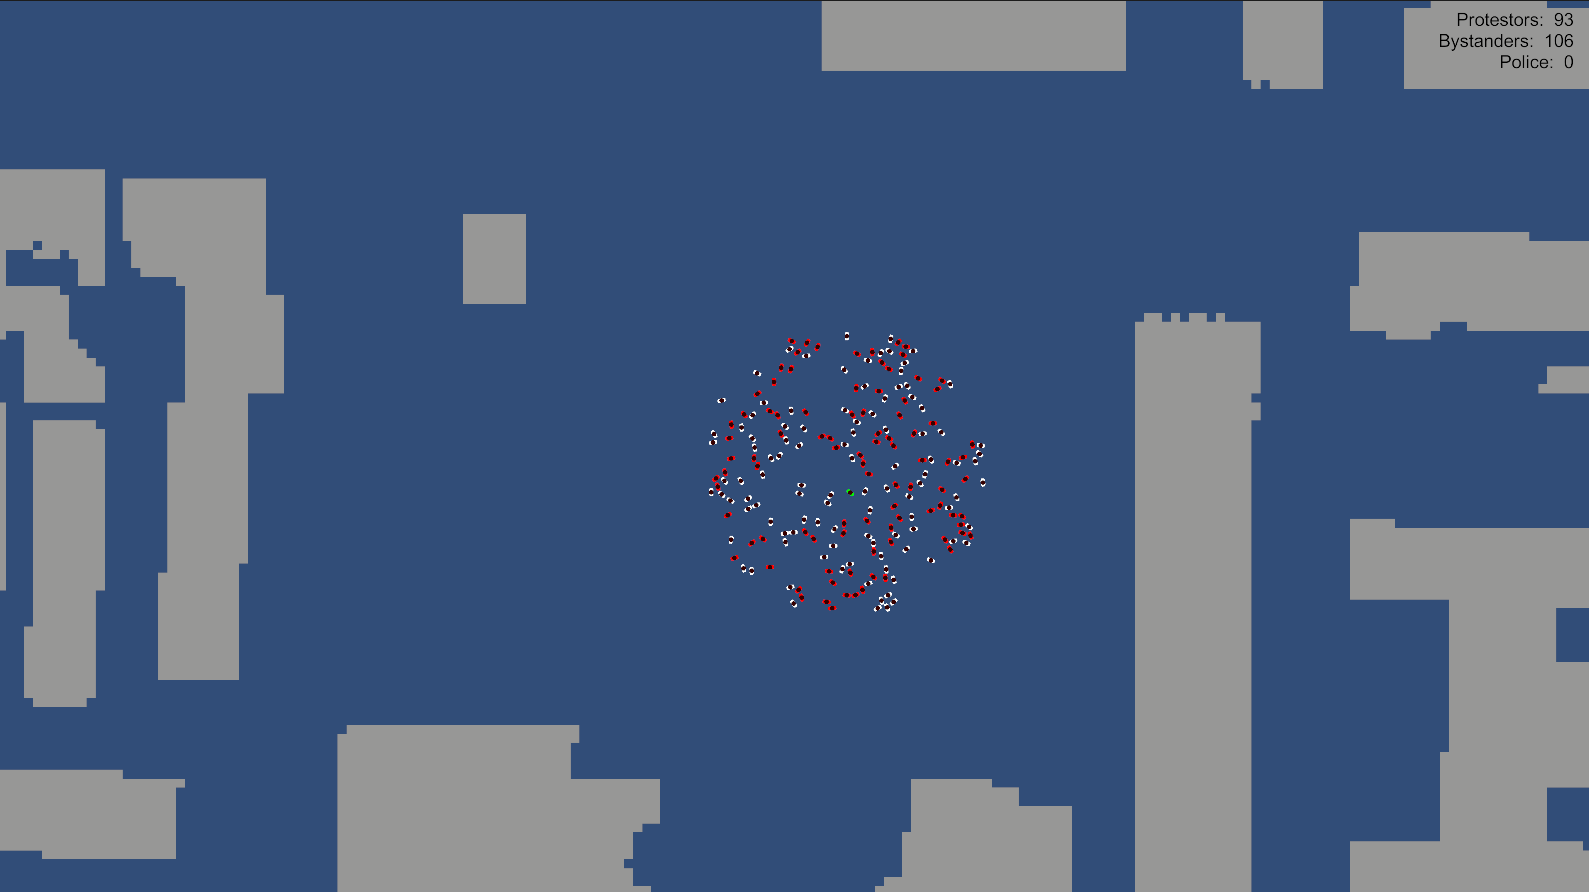
\includegraphics[width=0.95\columnwidth]{before.png}
  \caption{State at the start of the simulation}
  \label{fig:sub1}
\end{subfigure}%
\begin{subfigure}{.5\textwidth}
  \centering
  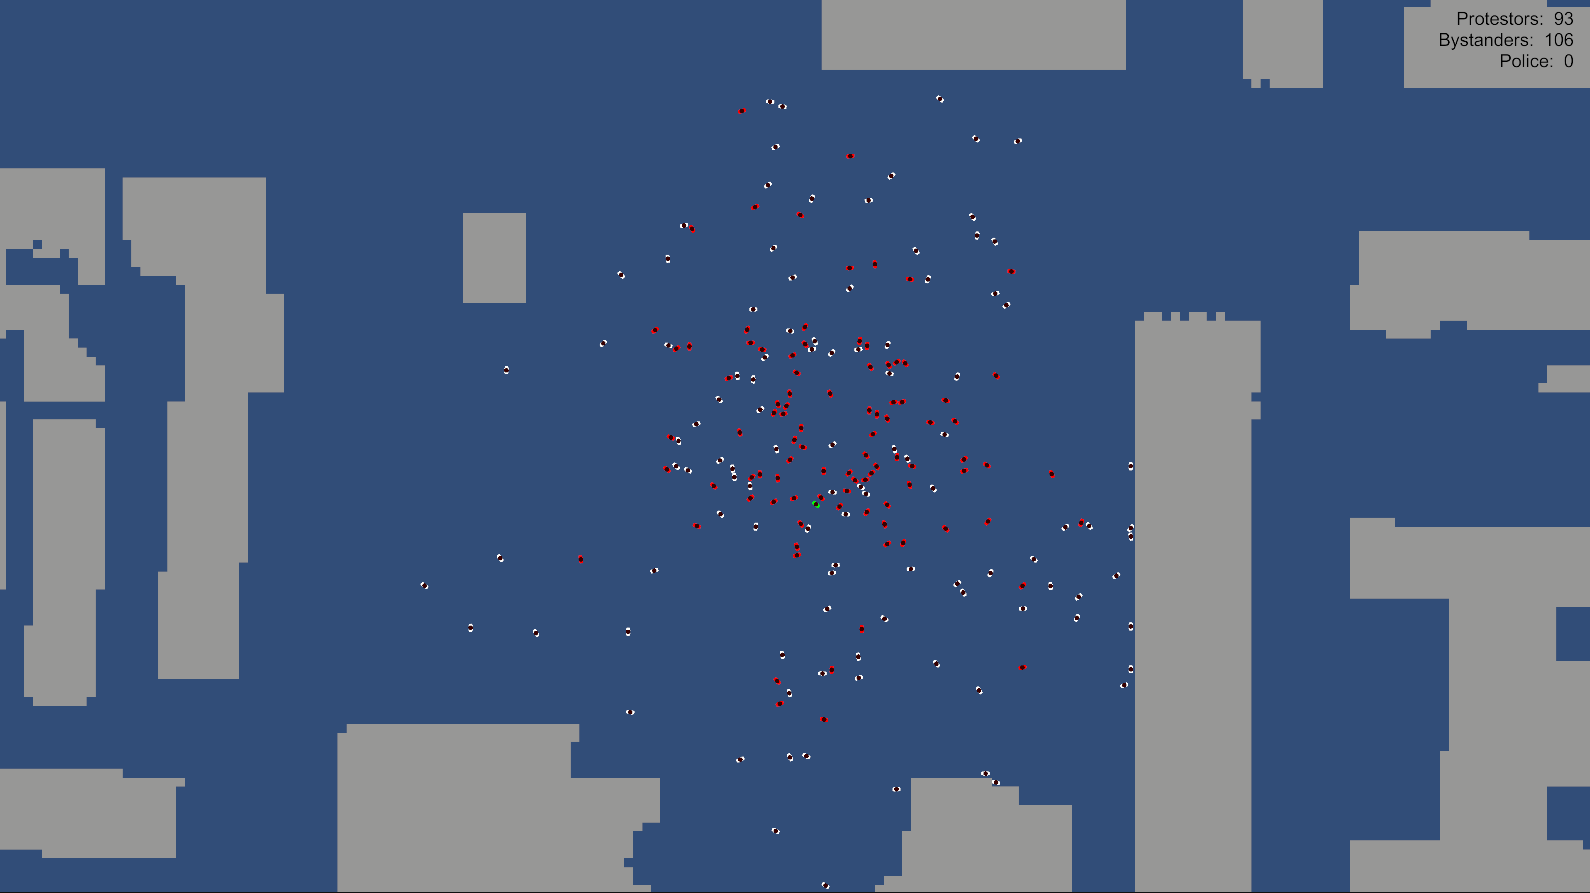
\includegraphics[width=0.95\columnwidth]{after.png}
  \caption{State after end-position-seeking-behaviour}
  \label{fig:sub2}
\end{subfigure}
\caption{Example of the effects of end-position-seeking-behaviour.}
\label{fig3}
\end{figure}

Leader Identification Time Interval is set to 1.5 by default to ensure that the simulation starts without a leader, so that we can observe how it emerges. Once the leader identifies, the nearby agents gradually begin to follow and form a hierarchy as shown in figure \ref{follow}. The formed group moves seamlessly around the map and successfully avoids arbitrarily placed police barricades. 

\begin{figure}[H]
\centering
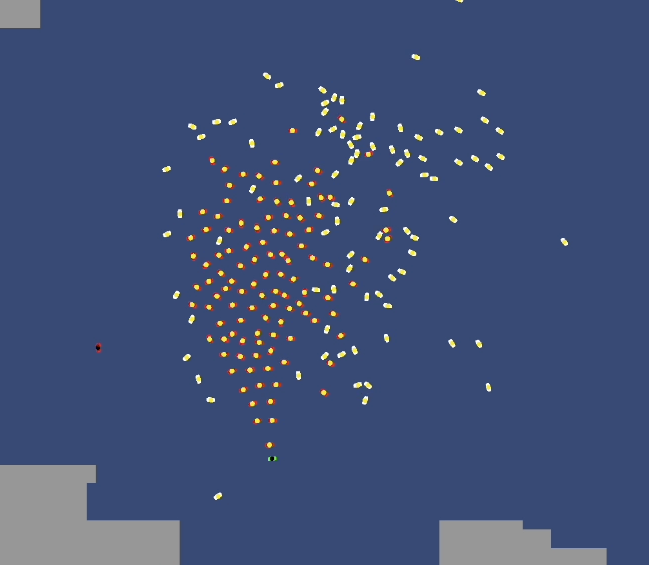
\includegraphics[width=0.95\columnwidth]{followleader.png}
\caption{Example of leader following behaviour: leader (green), following protesters (orange), bystanders (white) and a regular protester who is looking away and therefore not joining yet (red).}
\label{follow}
\end{figure}

\bigskip
We also observed various situations in which the leader unidentifies itself when the number of its followers is small enough for a long enough period of time. This causes a chain reaction that eventually leads to a complete dispersal of all actively following agents. However, some still remain protesters and a new leader can eventually emerge again. 

\section*{Discussion}

Most of the goals of the project were accomplished successfully, however we propose some potential improvements that are yet to be implemented: 
\begin{itemize}
\item current implementation of the map assumes buildings are the only structure that acts as a repulsive force on the agents. To increase realism, it would be necessary to also include other objects, such as trees, statues, etc.
\item solving the problem of displaying the agents' dimensions relative to building's dimensions (i.e. how to simultaneously show a big portion of the map while maintaining a clear vision of the agents).
\item developing an approach for police agents to find more optimal formations other than static barricade-like structures (e.g. by using genetic algorithms). 
\item introducing some uncertainty into vision might further improve the realism of the simulation - an agent should occasionally incorrectly recognize a protester as a bystander or vice versa, with a low, but non-zero probability. 
\end{itemize}

The entire code and other materials related to the project are publicly available at \url{https://github.com/bajicluka01/CollectiveBehaviour-GroupA}.

\acknow{NČ implemented agent movement, vision and interaction between different groups, PNM created the map and implemented the police agents, PM implemented transitions between groups (emotional contagion) and improved the visualization, LB did image processing for the map, implemented the baseline model and wrote the reports}
\showacknow % Display the acknowledgments section

% \pnasbreak splits and balances the columns before the references.
% If you see unexpected formatting errors, try commenting out this line
% as it can run into problems with floats and footnotes on the final page.
%\pnasbreak

\begin{multicols}{2}
\section*{\bibname}
 %Bibliography
\bibliography{./bib/bibliography}
\end{multicols}

\end{document}